\documentclass{article}

\usepackage[margin=1in]{geometry}
\usepackage{amsmath}
\usepackage{spverbatim}
\usepackage{graphicx}

\begin{document}
	
\title{ESOF 322 - Homework 3}
\author{Nathan Stouffer and Kevin Browder}

\maketitle
\newpage

\section*{Exercise 1}
We chose to combine the Strategy and Adapter Patterns.

\subsection*{Part A}
The UML Class Diagram is shown below. \\
\begin{figure}[h]
	\centering
	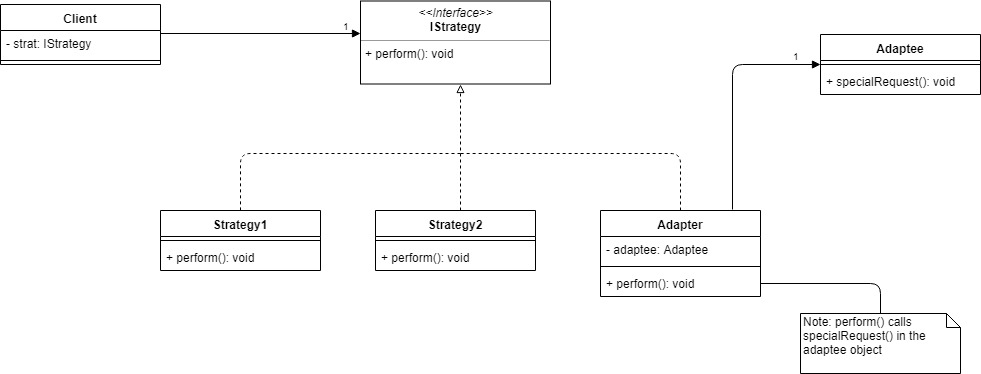
\includegraphics[width=6in]{hw3-class-diagram.jpg}
\end{figure}

\subsection*{Part B}
The UML Sequence Diagrams are shown below. The following image is from the perspective of the Strategy Pattern.
\begin{figure}[h]
	\centering
	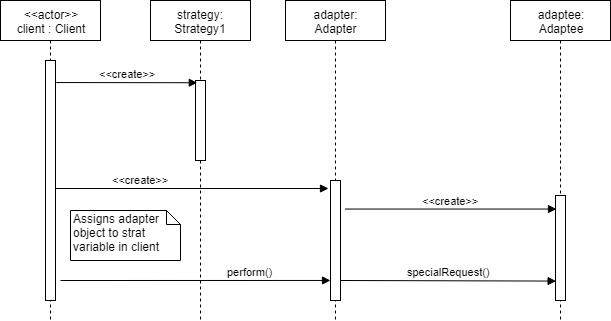
\includegraphics[width=5in]{hw3-strat-sequence.jpg}
\end{figure}
\newpage
This image is from the perspective of the Adapter Pattern.
\begin{figure}[h]
	\centering
	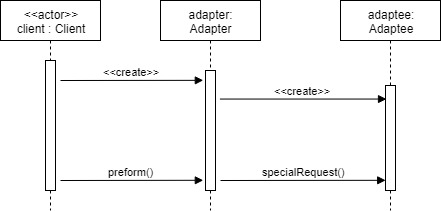
\includegraphics[width=5in]{hw3-adapt-sequence.jpg}
\end{figure}
\newpage

\section*{Exercise 2}

\subsection*{Part A}
Problem: Assume during your team's last sprint, that they completed 32 story points using a 3-person team working in sprints of 3 weeks for a total of 45-man days. Calculate your team's estimated velocity for the next sprint if we still have 3-week sprints, but you now added 2 engineers to the team, and one of them can only work 80\% of the time. \\\\
Solution: We estimate our focus factor using the equation
$$\text{actual velocity} = \text{ man days } * \text{ focus factor},$$
which can be rewritten as
$$\text{focus factor} = \dfrac{\text{actual velocity}}{\text{man days}}.$$
Plugging in our values, we find that focus factor
$= \dfrac{32}{45} = 0.7111$.
We now note that estimated velocity is predicted to be 
$$\text{estimated velocity} \approx \text{man days} * \text{focus factor}.$$
Additionally, our man days must now agree with the new number of engineers on the team. We will add 15 man days for the engineer that is able to work the full sprint and 
$0.8 * 15 = 12$
man days for the engineer that is able to work
$80\%$
of the time. This gives 72 man days. Thus,
$\text{estimated velocity} \approx \text{man days} * \text{focus factor} = 72 * 0.7111 = 51.2$.
Since we must have an integer number of story points, our estimated velocity translates to 51 story points in the next sprint.

\subsection*{Part B}
Problem: How would you estimate a focus factor for a brand-new team? \\\\
Solution: We should estimate a focus factor for a brand-new team as $70\%$.

\subsection*{Part C}
Problem: We looked at using poker semi-Fibonacci sequences to estimate story points. Think of another way to estimate story points and explain it. Is it better or worse than poker? \\\\
Solution: Another method of estimating story points would be to separately ask the project leader and the three most experienced engineers to estimate the story points of each item in the backlog. We then average their responses (rounding up to the nearest integer) and assign that number of story points to the item. \\\\
This method is worse than poker semi-Fibonacci for two reasons.
First, there are engineers pertinent to the project that are not involved in the estimation process. A good method for estimation would include the input of all engineers involved in the project to output the best estimation.
Second, our method is not iterative. The estimations are made based off one-time decisions and are never reviewed. In the poker semi-Fibonacci method, engineers must reach a consensus through discussion and recasting votes.

\subsection*{Part D}
Problem: Draw a UML class diagram of a binary tree. Each node contains an integer. \\\\
Solution: The UML class diagram is shown below.
\begin{figure}[h]
	\centering
	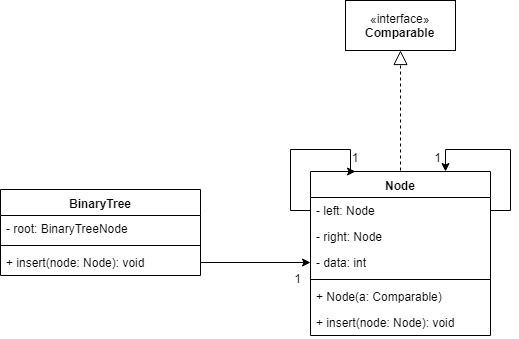
\includegraphics[width=5in]{hw3-binary-tree.jpg}
\end{figure}

\subsection*{Part E}
Problem: Provide the corresponding object-oriented code that implements your binary tree design from part D. \\\\
Solution: The code structure for a binary tree is shown below
\begin{spverbatim}
class Node implements Comparable {
	
    private int data;
    private Node left, right;
	
    public Node(int item) {
        data = item;
        left = right = null;
    }
	
    /**
    * Compares current node value with input node
    * returns 1 if input is greater than current node
    * returns -1 if input is less than current node
    * @param input
    * @return 
    */
    @Override
    public int compareTo(Object input) {
        Node node = (Node) input;
        if (node.data > this.data) {
            return 1;
        }
        else {
            return -1;
        }
    }
	
    public void insert(Node node) {
        if (compareTo(node) == 1) {
            if (this.right == null) {
                 this.right = node;
            }
            else {
                 this.right.insert((node));
            }
        } else {
            if (this.left == null) {
                this.left = node;
            }
            else {
                this.left.insert(node);
            }
        }
    }
	
    public int getData() {
        return data;
    }
	
    public void setData(int data) {
        this.data = data;
    }
}
\end{spverbatim}

\newpage
\begin{spverbatim}
/**
* Class to represent a binary tree
*/
class BinaryTree {
	
    // Root of Binary Tree 
    Node root;
	
    BinaryTree(int key) {
        root = new Node(key);
    }
	
    BinaryTree() {
        root = null;
    }
	
	
    public void insert(Node node){
        if(root == null){
            root = node;
        }
        else{
            root.insert(node);
        }
    }
}
\end{spverbatim}
\newpage

\subsection*{Part F}
Problem: Draw a UML class diagram of a linked list that contains Employee records as data. An Employee record has a name, a social security number, and a salary. \\\\
Solution: The UML is shown below.
\begin{figure}[h]
	\centering
	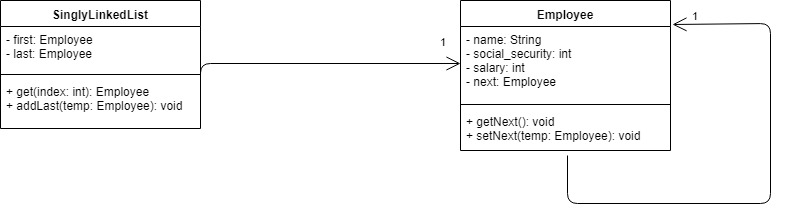
\includegraphics[width=5in]{hw3-linked-list.jpg}
\end{figure}

\subsection*{Part E}
Problem: Provide the corresponding object-oriented code that implements your linked list from part F. \\\\
Solution: The code is shown below.
\begin{spverbatim}
public class SinglyLinkedList {
	
    // global variables pointin to the first
    // and last values in the list
    private Employee first;
    private Employee last;
	
    /**
    * constructor to initiliaze global variables
    */
    SinglyLinkedList(){
        this.first = null;
        this.last = null;
    }
	
    /**
    * method to return the element of a SinglyLinkedList at index
    * @param index
    * @return 
    */
    public Employee get(int index){
        if (last == null){ return null; }
        else{
            Employee iter = first;
            for (int i = 0; i < index; i++){ iter = iter.getNext(); }
            return iter;
        }
    }
	
    /**
    * method to add an element to the end of a SinglyLinkedList
    * @param temp 
    */
    public void addLast(Employee temp){
        // check is list is empty, make tempt the first element
        if (last == null){
            this.first = temp;
            this.last = temp;
        }
        // otherwise, add temp to the end
        else{
            last.setNext(temp);
            last = temp;
        }
    }
	
}
\end{spverbatim}

\newpage
\begin{spverbatim}
public class Employee {
	
    // global variables with information about the Employee
    private String name;
    private int social_security;
    private int salary;
    // next element in linked list
    private Employee next = null;
	
    /**
    * constructor to initialize global variables
    * @param name
    * @param social_security
    * @param salary 
    */
    Employee(String name, int social_security, int salary){
        this.name = name;
        this.social_security = social_security;
        this.salary = salary;
    }
	
    /**
    * method to set the next element in the linked list
    * @param temp 
    */
    public void setNext(Employee temp){ this.next = temp; }

    /**
    * method to return the next element in the linked list
    * @return 
    */
    public Employee getNext(){ return this.next; }
	
    /**
    * method to return the information of the employee
    * @return 
    */
    @Override
    public String toString(){ 
        return "name: " + name + " social security: " + Integer.toString(social_security)
        + " salary: " + Integer.toString(salary) + "\n";
    }
}
\end{spverbatim}

\end{document}